\section{壱岐から上げた場合}
\label{sec:iki}

\subsection{地上気象の資料で結果が変わる}
\label{sec:amedas}

壱岐は面積約 \SI{130}{\square\kilo\metre} の島で、ERA5 の \ang{0.25} 格子では島のある格子の
\SI{96}{\percent} 以上が海になる。そのまま使うと海上の風になり、9 時に風が
\SI{5}{\metre\per\second} 以下の日は \SI{27}{\percent} しかない（格子の中央値 \SI{6.9}{\metre\per\second}）。
本文の地図と表では、これを避けるために最寄りの「陸が半分以上の格子」を使った。
壱岐の場合、その格子は約 \SI{40}{\kilo\metre} 離れた唐津市の内陸にある。

どちらが実際に近いかを確かめるため、壱岐の芦辺と、平戸・唐津のアメダスの 9 時の観測
（903 日）と比べた（図~\ref{fig:amedas}）。
\begin{itemize}
  \item 芦辺で 9 時の地上気象が打ち上げに向く日は \SI{77}{\percent}（風 \SI{5}{\metre\per\second} 以下が \SI{86}{\percent}、
    降水なしが \SI{89}{\percent}、風速の中央値 \SI{2.8}{\metre\per\second}）。
    ERA5（最寄りの陸の格子）では \SI{59}{\percent}、島の格子そのままでは \SI{24}{\percent} だった。
  \item 平戸（観測 \SI{75}{\percent}、ERA5 \SI{70}{\percent}）と唐津（観測 \SI{81}{\percent}、ERA5 \SI{70}{\percent}）でも
    ERA5 は観測より低い。ERA5 だけで評価すると、実施できる確率は控えめに出る。
  \item 日ごとの判定は、観測と ERA5 で \SI{76}{\percent} の日に一致した（芦辺）。外れた日の大半は
    「観測では向くが ERA5 では向かない」日（\SI{21}{\percent}）で、逆は \SI{3}{\percent} だった。
\end{itemize}

アメダスの風速計は地上 \SI{10}{\metre} 前後の高さにあり、周囲の地形や建物の影響も受ける。
打ち上げ場所の風と同じではないが、\SI{25}{\kilo\metre} 格子の再解析よりは打ち上げ場所に近い。
そこで\textbf{壱岐については、地上気象をアメダス芦辺の観測で判定した値を最良の推定とする}。
近くにアメダスのある平戸・大島と唐津の 2 地点も同じように計算し直した（表~\ref{tab:amedas}）。

\begin{table}[htbp]
\centering
\scriptsize
\caption{地上気象をアメダスの 9 時の観測で判定した場合。ERA5 の列は本文の地図と表~\ref{tab:sites} の値。
観測が欠けた日（各地点 1--4 日）は ERA5 の判定を使った。}
\label{tab:amedas}
\resizebox{\linewidth}{!}{\begin{tabular}{llrrrcrc}
\toprule
& & \multicolumn{2}{c}{地上気象が向く [\%]} & \multicolumn{4}{c}{実施できる [\%]} \\
& & & & \multicolumn{2}{c}{標準} & \multicolumn{2}{c}{短時間} \\
候補地 & アメダス & ERA5 & アメダス & ERA5 & アメダス (95\% 区間) & ERA5 & アメダス (95\% 区間) \\
\midrule
壱岐（島の中央） & 芦辺 & 59 & 77 & 29 & \textbf{37} (34--40) & 38 & \textbf{49} (46--51) \\
平戸・大島 & 平戸 & 70 & 75 & 33 & \textbf{34} (31--38) & 34 & \textbf{38} (34--41) \\
唐津・加唐島 & 唐津 & 70 & 81 & 32 & \textbf{36} (33--39) & 45 & \textbf{52} (50--55) \\
唐津・相知 & 唐津 & 81 & 81 & 23 & \textbf{23} (20--27) & 42 & \textbf{43} (40--45) \\
\bottomrule
\end{tabular}
}
\end{table}

\begin{figure}[htbp]
\centering
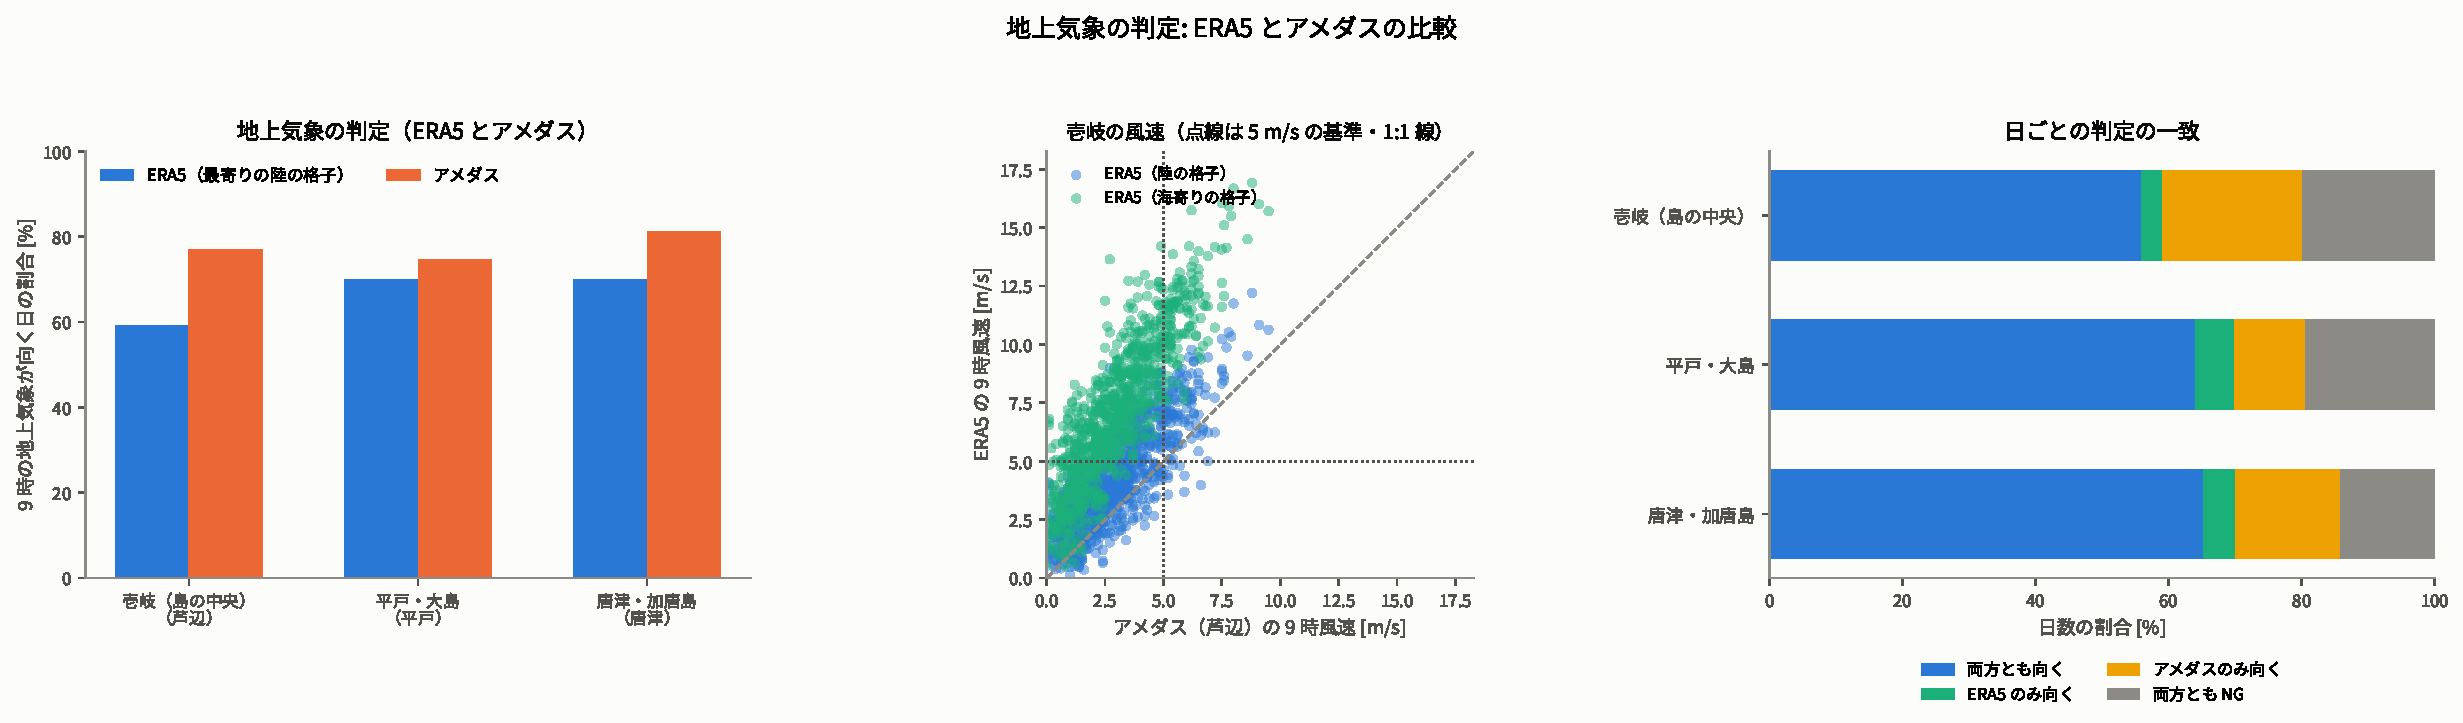
\includegraphics[width=\linewidth]{amedas_compare.pdf}
\caption{9 時の地上気象の比較。(a) 打ち上げに向く日の割合（ERA5 とアメダス）。
(b) 壱岐の 9 時の風速（ERA5 とアメダス芦辺）。(c) 日ごとの判定の一致。}
\label{fig:amedas}
\end{figure}

\subsection{壱岐で実施できる確率と、できない確率}

アメダスで地上気象を判定すると、壱岐から上げて実施できる確率は
\begin{itemize}
  \item 標準の飛行で \textbf{\SI{37}{\percent}}（95\% 区間 34--40）、実施できない確率は \SI{63}{\percent}
  \item 短時間の飛行で \textbf{\SI{49}{\percent}}（46--51）、実施できない確率は \SI{51}{\percent}
\end{itemize}
である。アメダスで計算し直した 4 地点の中では、標準の飛行で最も高い（ただし唐津・加唐島の \SI{36}{\percent} との差は区間の中にある）。
短時間の飛行では唐津・加唐島（\SI{52}{\percent}）とほぼ並ぶ。
つまり\textbf{壱岐は、冬の打ち上げ場所として日本で最も条件の良い場所の 1 つ}である。

実施できない日の内訳を表~\ref{tab:iki} に示す。標準の飛行では、
落下予測が山地（主に山口・福岡・広島の山地）に入って見送る日が \SI{35}{\percent} で最も多く、
地上の風・雨で中止する日が \SI{22}{\percent}、打ち上げ地点の雪は \SI{2}{\percent} である。
短時間の飛行にすると、山地に入る日が \SI{24}{\percent} に減る。

\begin{table}[htbp]
\centering
\small
\caption{壱岐（島の中央、33.78, 129.72）で毎朝 9 時に判断したときの結果の内訳（903 日の割合）。
雪 → 地上気象 → 落下予測の順に判断した。右の列は地上気象を ERA5 で判定した場合。}
\label{tab:iki}
\begin{tabular}{lrrr}
\toprule
& \multicolumn{2}{c}{地上気象: アメダス芦辺} & ERA5 \\
9 時の判断の結果 & 標準 [\%] & 短時間 [\%] & 標準 [\%] \\
\midrule
成功: 瀬戸内海に落ちる & 32.6 & 41.2 & 25.7 \\
成功: 平野に落ちる & 3.2 & 6.2 & 2.5 \\
成功: 海岸から 3 km 以内の海 & 1.2 & 1.2 & 0.9 \\
中止: 打ち上げ地点に雪 & 2.1 & 2.1 & 2.1 \\
中止: 地上の風・雨 & 22.4 & 22.4 & 39.2 \\
見送り: 落下予測が山地 & 35.1 & 24.1 & 27.3 \\
見送り: 落下予測が沖の海 & 2.2 & 1.5 & 1.5 \\
見送り: 落下予測が市街地 & 1.0 & 1.1 & 0.7 \\
見送り: 落下予測地点に雪 & 0.2 & 0.2 & 0.1 \\
\midrule
実施できる（成功の合計） & \textbf{36.9} & \textbf{48.6} & 29.1 \\
\quad 95\% 区間 & 34--40 & 46--51 & 26--32 \\
実施できない & 63.1 & 51.4 & 70.9 \\
\bottomrule
\end{tabular}

\end{table}

\begin{figure}[htbp]
\centering
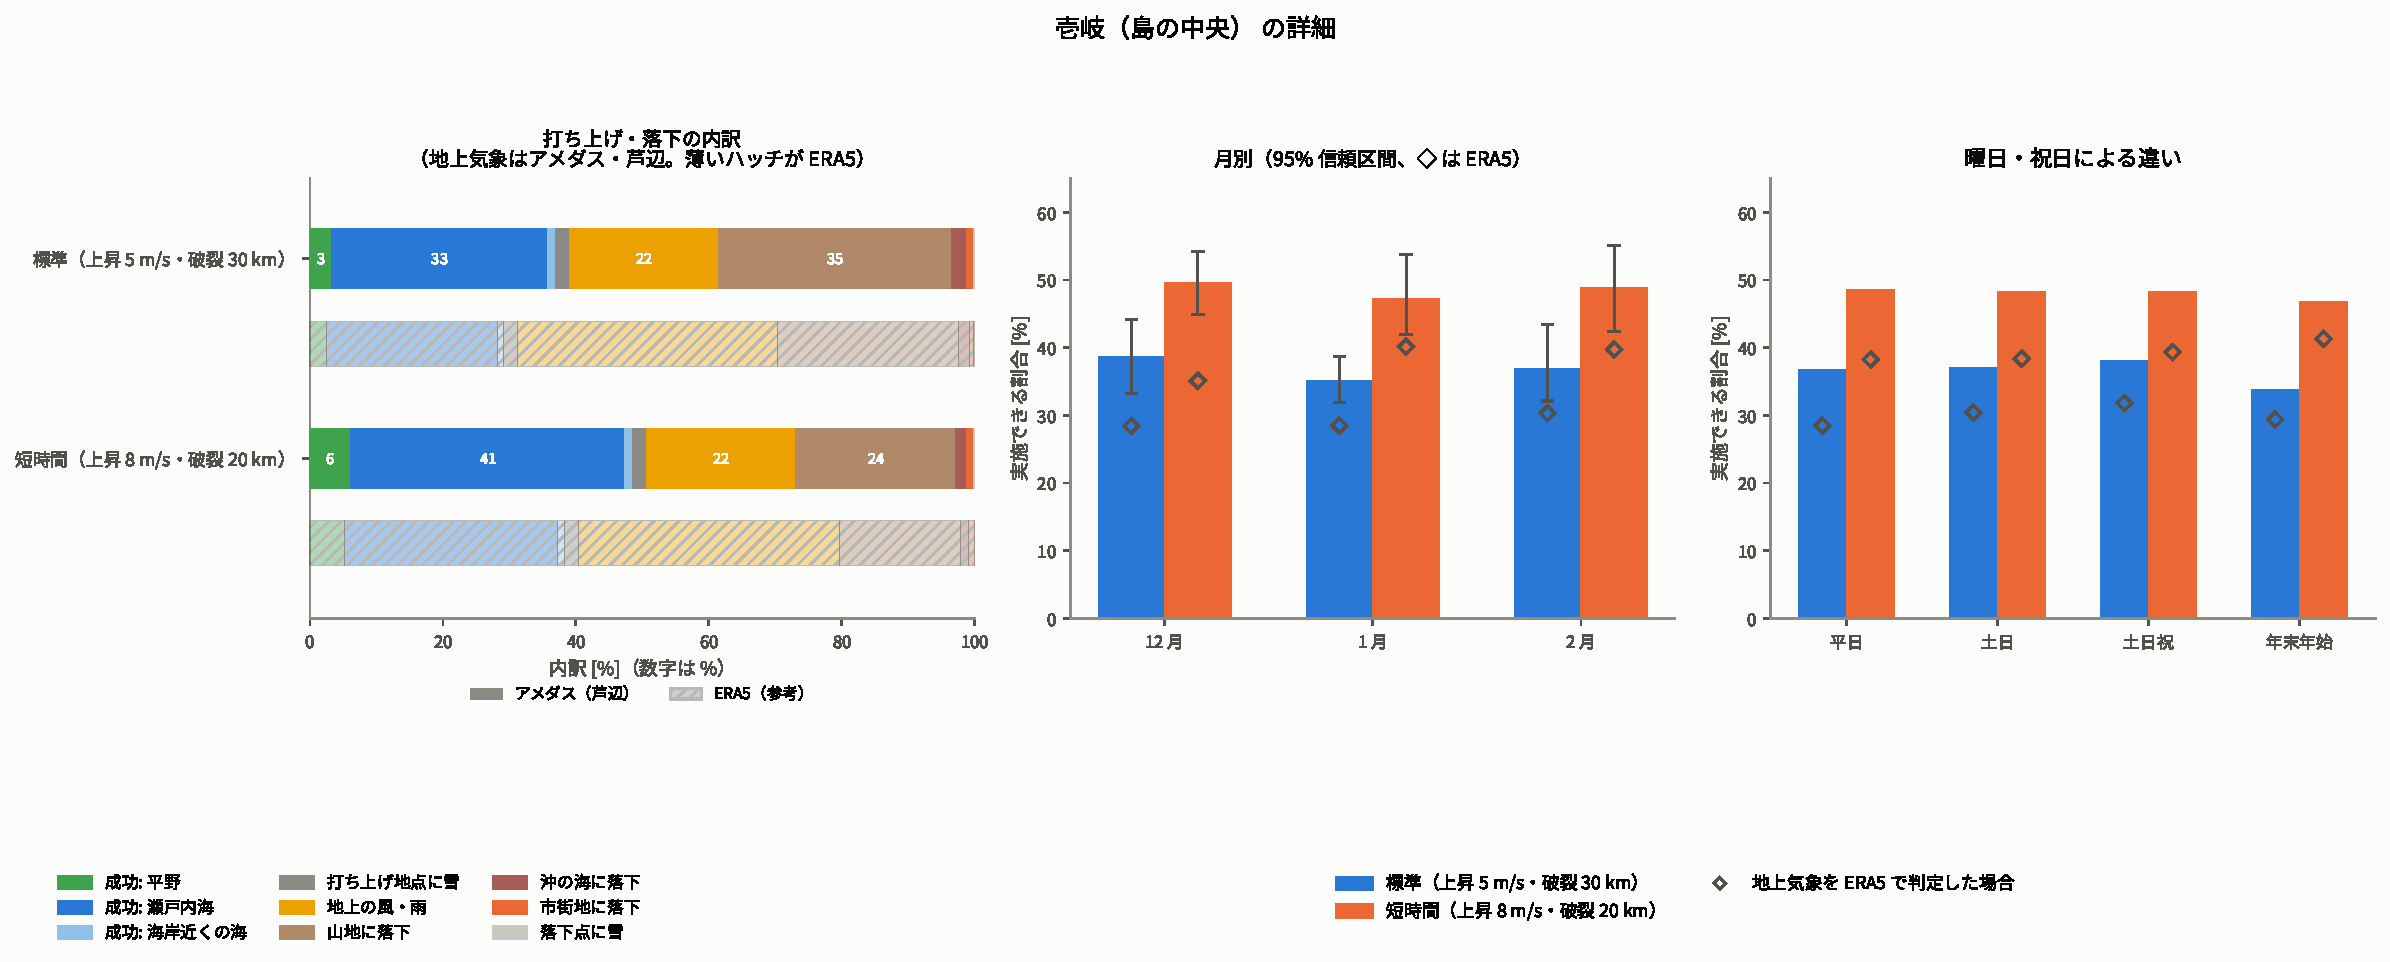
\includegraphics[width=\linewidth]{iki_detail.pdf}
\caption{壱岐の詳細（地上気象はアメダス芦辺）。(a) 9 時の判断の結果の内訳。
(b) 月ごとの実施できる確率（95\% 区間つき）。(c) 平日・土日・土日祝・年末年始の確率。
薄い色は地上気象を ERA5 で判定した場合。}
\label{fig:iki}
\end{figure}

\subsection{壱岐のどこで上げるか}

壱岐島の中で打ち上げに使えそうな広場は 34 か所あり、電線・建物・林から \SI{60}{\metre} 以上
離れられる所は 10 か所ある（図~\ref{fig:spotsiki}、表~\ref{tab:spotsiki}）。
島の中でどこから上げても、実施できる確率は標準の飛行で \SIrange{36}{38}{\percent}、
短時間の飛行で \SIrange{45}{50}{\percent} と、ほとんど変わらない。
壱岐空港（島の南東）の周り \SI{3}{\kilo\metre} は除いた。空港から \SI{9}{\kilo\metre} 以内の所は、
飛行の許可を取るときに空港との調整が要る可能性がある。

\begin{figure}[htbp]
\centering
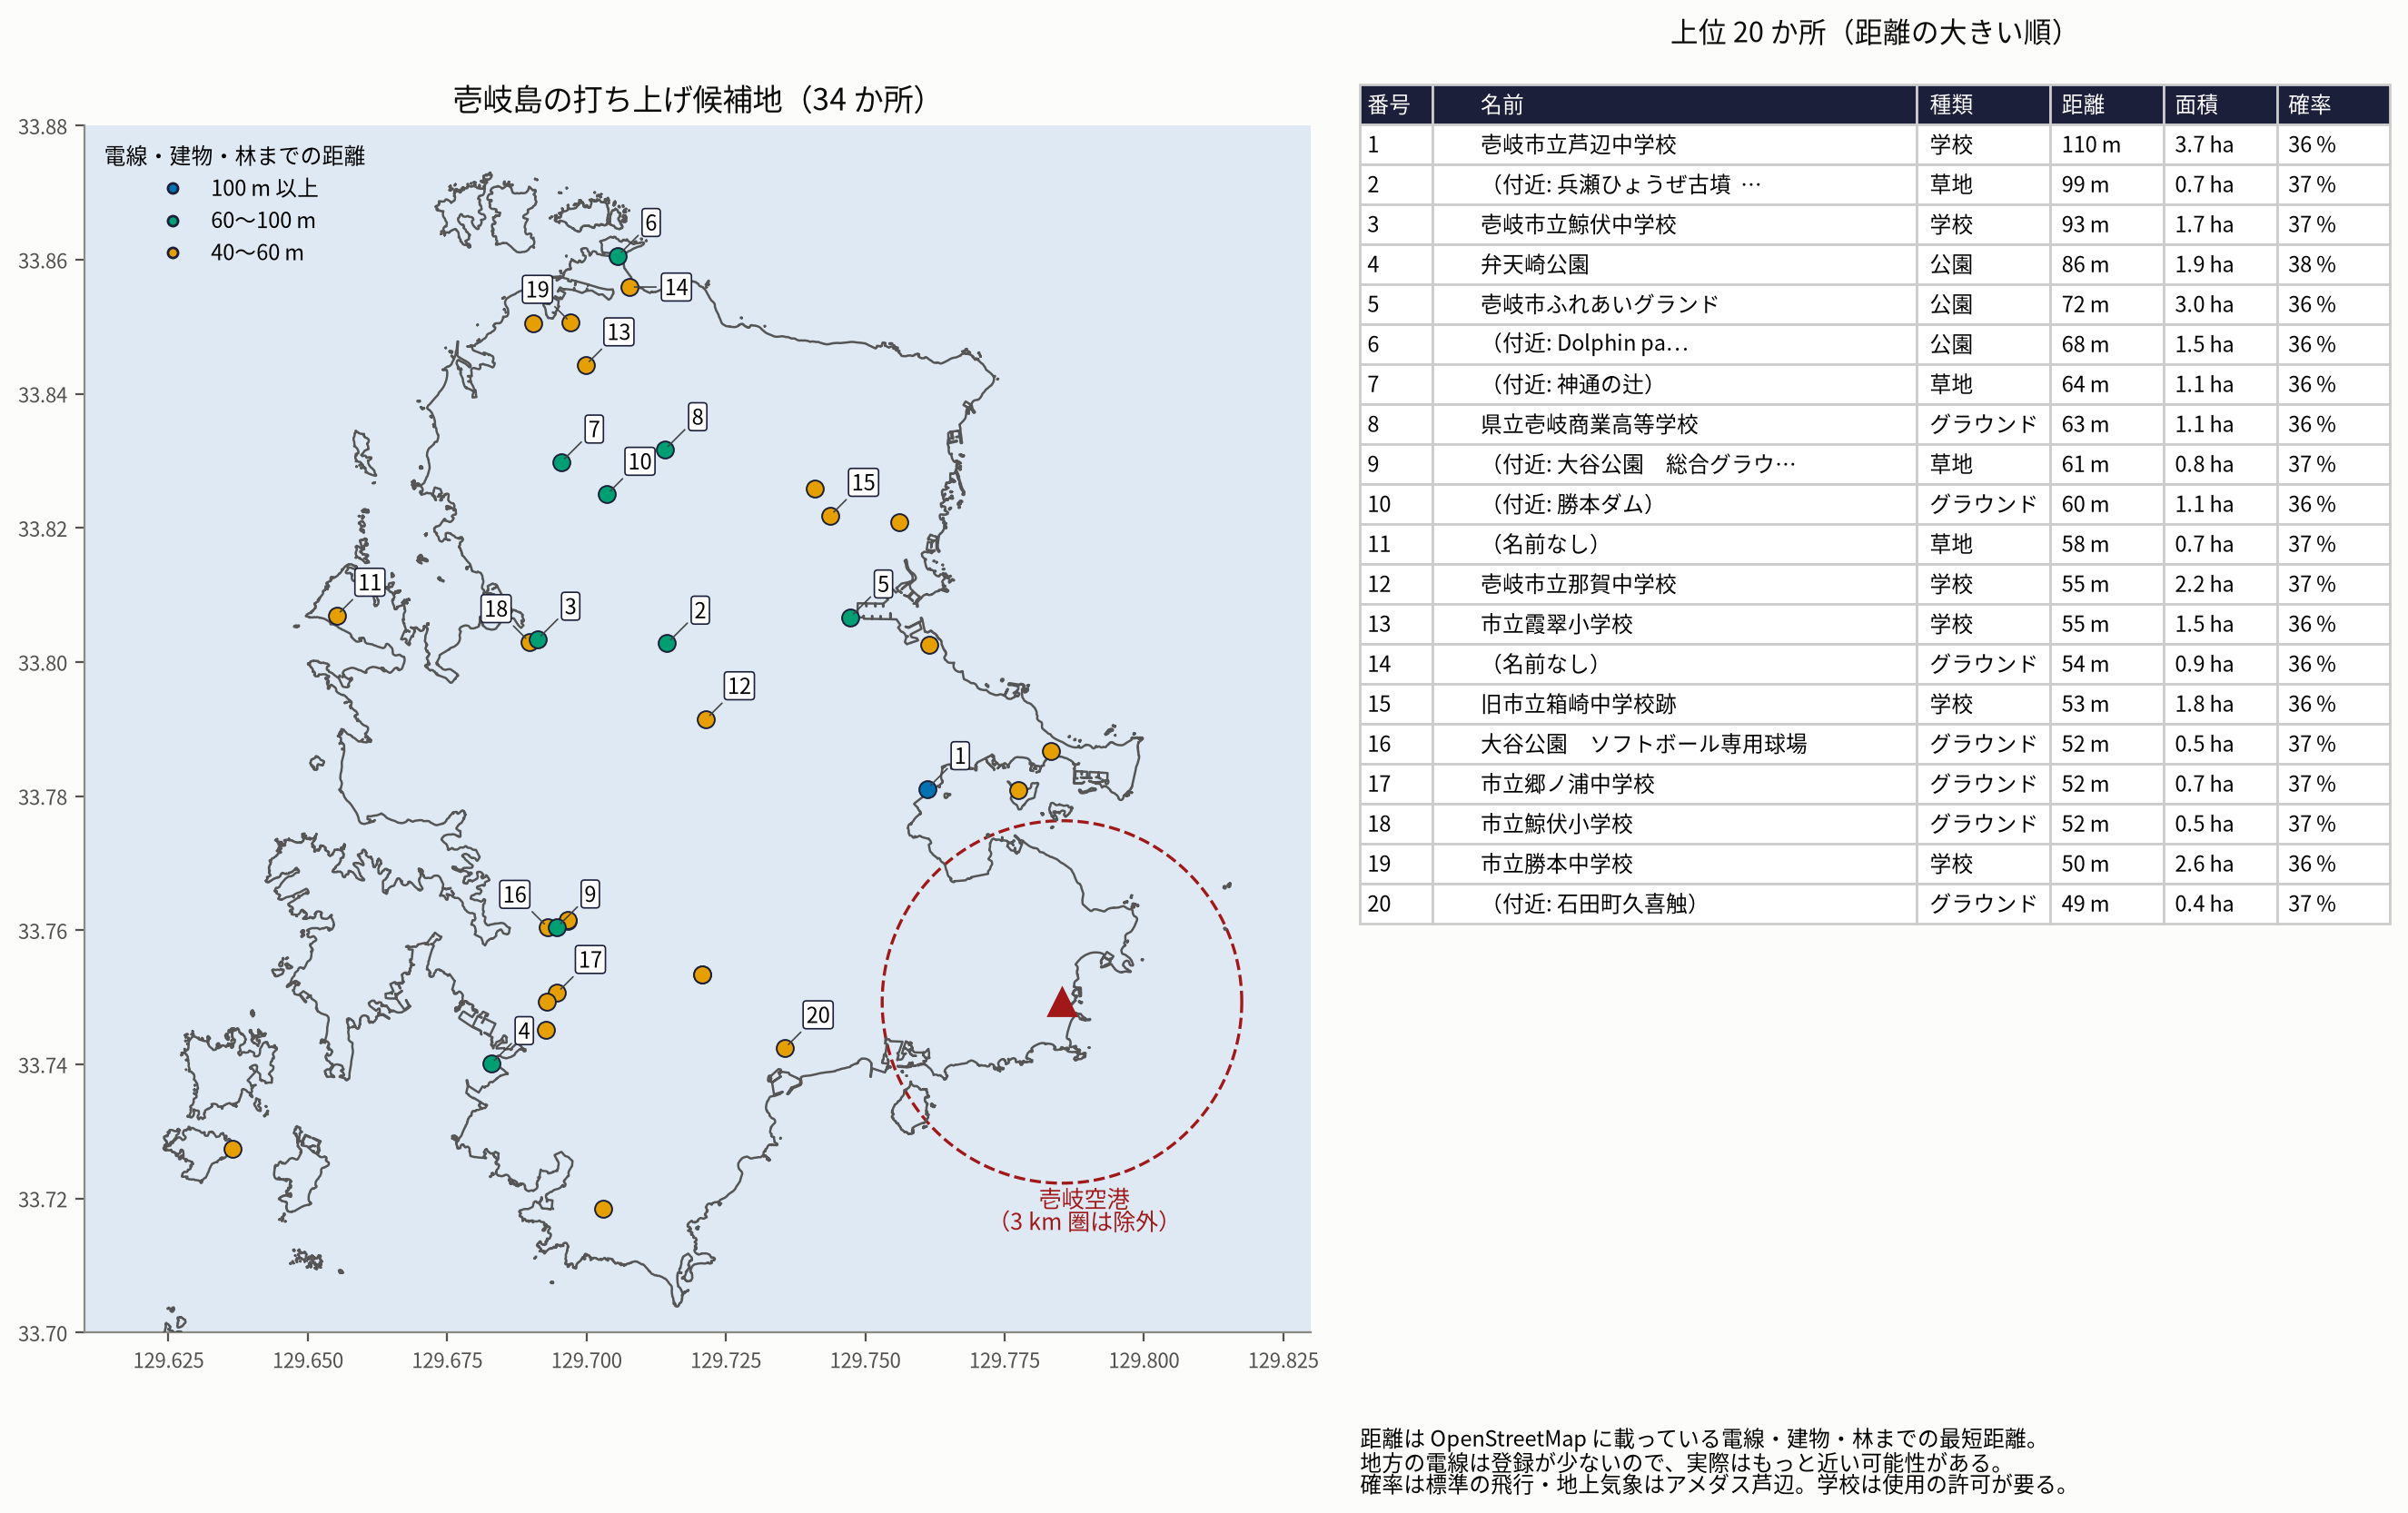
\includegraphics[width=\linewidth]{launch_spots_iki.png}
\caption{壱岐島の打ち上げ候補地。色は電線・建物・林までの距離。番号は右の一覧と対応する。
確率は標準の飛行、地上気象はアメダス芦辺。}
\label{fig:spotsiki}
\end{figure}

\begin{table}[htbp]
\centering
\scriptsize
\caption{壱岐島の打ち上げ候補地（距離の大きい順に 15 か所）。「距離」は電線・建物・林までの距離、
「空港」は壱岐空港の滑走路までの距離、確率は標準 / 短時間の飛行。名前が「付近:」の所は
OpenStreetMap に名前が無く、近くの地名を付けた。}
\label{tab:spotsiki}
\resizebox{\linewidth}{!}{\begin{tabular}{rllcrrrcl}
\toprule
 & 名前 & 種類 & 緯度, 経度 & 距離 [m] & 面積 [ha] & 空港 [km] & 確率 [\%] & \\
\midrule
1 & 壱岐市立芦辺中学校 & 学校 & 33.7811, 129.7611 & 110 & 3.7 & 3.8 & 36 / 49 & 要許可（学校） \\
2 & （付近: 兵瀬ひょうぜ古墳  前方後円墳） & 草地 & 33.8028, 129.7145 & 99 & 0.7 & 8.6 & 37 / 48 &  \\
3 & 壱岐市立鯨伏中学校 & 学校 & 33.8034, 129.6912 & 93 & 1.7 & 10.4 & 37 / 47 & 要許可（学校） \\
4 & 弁天崎公園 & 公園 & 33.7401, 129.6829 & 86 & 1.9 & 9.4 & 38 / 49 &  \\
5 & 壱岐市ふれあいグランド & 公園 & 33.8067, 129.7473 & 72 & 3.0 & 6.9 & 36 / 48 &  \\
6 & （付近: Dolphin park） & 公園 & 33.8606, 129.7056 & 68 & 1.5 & 14.0 & 36 / 45 &  \\
7 & （付近: 神通の辻） & 草地 & 33.8298, 129.6954 & 64 & 1.1 & 11.9 & 36 / 46 &  \\
8 & 県立壱岐商業高等学校 & グラウンド & 33.8316, 129.7140 & 63 & 1.1 & 10.9 & 36 / 46 & 要許可（学校） \\
9 & （付近: 大谷公園　総合グラウンド） & 草地 & 33.7605, 129.6947 & 61 & 0.8 & 8.5 & 37 / 49 &  \\
10 & （付近: 勝本ダム） & グラウンド & 33.8250, 129.7036 & 60 & 1.1 & 11.0 & 36 / 46 &  \\
11 & （名前なし） & 草地 & 33.8069, 129.6552 & 58 & 0.7 & 13.5 & 37 / 47 &  \\
12 & 壱岐市立那賀中学校 & 学校 & 33.7915, 129.7215 & 55 & 2.2 & 7.3 & 37 / 48 & 要許可（学校） \\
13 & 市立霞翠小学校 & 学校 & 33.8443, 129.6999 & 55 & 1.5 & 12.8 & 36 / 46 & 要許可（学校） \\
14 & （名前なし） & グラウンド & 33.8559, 129.7077 & 54 & 0.9 & 13.4 & 36 / 45 &  \\
15 & 旧市立箱崎中学校跡 & 学校 & 33.8218, 129.7437 & 53 & 1.8 & 8.5 & 36 / 47 & 要許可（学校） \\
\bottomrule
\end{tabular}
}
\end{table}

\subsection{壱岐の土日}

\begin{table}[htbp]
\centering
\scriptsize
\caption{壱岐の土日の確率（地上気象はアメダス芦辺）。数え方は \ref{sec:weekend} 節を参照。}
\label{tab:ikiweekend}
\resizebox{\linewidth}{!}{\begin{tabular}{lrrrrrrrrrr}
\toprule
& 全日 & 土日の & 決めた & 週末の & 土曜できた & \multicolumn{2}{c}{1 冬に実施できる [日]} & \multicolumn{3}{c}{毎週末挑戦して [\%]} \\
飛行 & [\%] & 1 日 [\%] & 土曜 [\%] & どちらか [\%] & 日曜も [\%] & 全日 & 土日 & 1 週目 & 2 週以内 & 4 週以内 \\
\midrule
標準 & 37 & 37 & 40 & 58 & 42 & 33.6 & 9.6 & 58 & 82 & 93 \\
短時間 & 49 & 48 & 53 & 71 & 49 & 44.3 & 12.7 & 72 & 92 & 98 \\
\bottomrule
\end{tabular}
}
\end{table}

壱岐（標準の飛行）では、土日の 1 日に実施できる確率が \SI{37}{\percent}、1 回の週末（土日の 2 日）の
どちらかで実施できる確率が \SI{58}{\percent} である（表~\ref{tab:ikiweekend}）。
12--2 月の 1 冬に実施できる日は平均 33.6 日、そのうち土日は 9.6 日ある。
毎週末挑戦すれば、2 週以内に \SI{82}{\percent}、4 週以内に \SI{93}{\percent} の確率で実施できる。
短時間の飛行なら、1 回の週末で \SI{71}{\percent}、2 週以内で \SI{92}{\percent} になる。

島で上げる場合は、機材と人をフェリーで運ぶ日程も週末に合わせる必要がある。
前日の予報で落下予測が山地に入ると分かった週末は、渡航そのものを見送ることになる。
